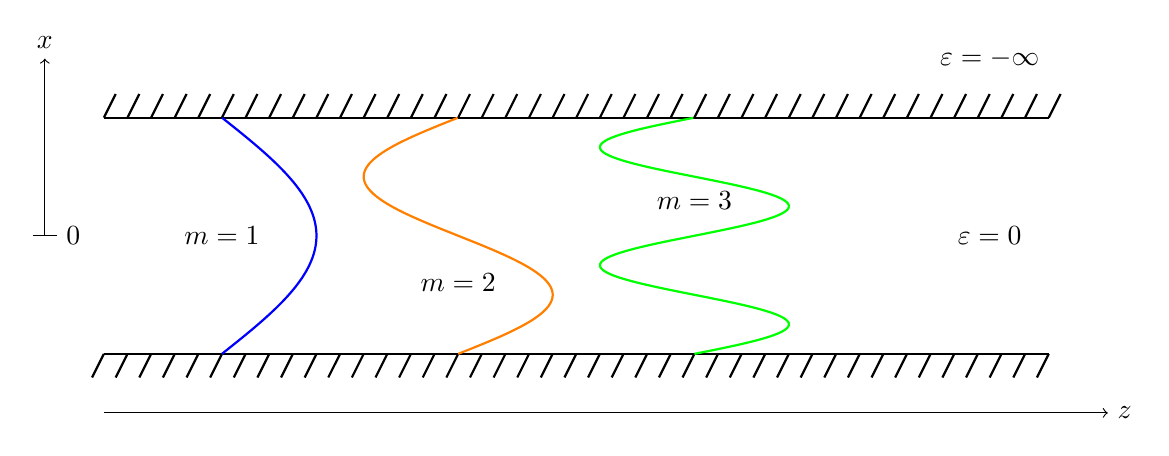
\begin{tikzpicture}[scale=1.5]

% -----------------------------
% Fiber walls (cladding)
% -----------------------------
\draw[thick] (0,0) -- (8,0);   % bottom wall
\draw[thick] (0,2) -- (8,2);   % top wall

% small hatch marks to mimic "/////"
\foreach \x in {0,0.2,...,8} {
    \draw[thick] (\x-0.1,-0.2) -- ++(0.1,0.2);
    \draw[thick] (\x,2) -- ++(0.1, 0.2);
}

% -----------------------------
% Mode 1 (fundamental)
% -----------------------------
\draw[blue, thick, smooth, samples=200, domain=0:2] 
    plot ({1 + 0.8*sin(pi/2*\x r)}, \x);  % single hump mode

% Mode 2 (first excited)
\draw[orange, thick, smooth, samples=200, domain=0:2] 
    plot ({3 + 0.8*sin(pi*\x r)}, \x);    % two humps mode

% Mode 3 (second excited)
\draw[green, thick, smooth, samples=200, domain=0:2] 
    plot ({5 + 0.8*sin(2*pi*\x r)}, \x);    % two humps mode
% -----------------------------
% Axes
% -----------------------------
\draw[->] (0,-0.5) -- (8.5,-0.5) node[right] {$z$};
\draw[->] (-0.5,1) -- (-0.5,2.5) node[above] {$x$};
\draw[-] (-0.6, 1) -- (-0.4, 1) node[right] {$0$};
% -----------------------------
% Labels
% -----------------------------
\node at (1,1) {$m=1$};
\node at (3,0.6) {$m=2$};
\node at (5,1.3) {$m=3$};
\node at (7.5, 2.5) {$\varepsilon=-\infty$};
\node at (7.5, 1) {$\varepsilon=0$};

\end{tikzpicture}
